\documentclass[11pt]{article}

\usepackage[margin=1in]{geometry}
\usepackage{amsmath,amssymb}
\usepackage{booktabs}
\usepackage{graphicx}
\usepackage{longtable}
\usepackage{hyperref}

\title{Spectral Dynamics, Null-Ladder Specificity, and Microtubule Telemetry: A Bounded Biology-Sidecar Release for HAOS-IIP}
\author{Tomislav Rupi\'c \\ Independent Researcher}
\date{April 2026}

\begin{document}

\maketitle

\begin{abstract}
This release documents a sidecar development cycle in HAOS-IIP: a spectral-address dynamics probe, a progressively hardened null ladder, and a first external toy-biology telemetry test on a microtubule-inspired cylindrical lattice. The internal graph dynamics improved recoverability and branch-identity scores after the local address term was replaced by a spectral projection term, but remained marginal under increasingly strict nulls. The null ladder now includes degree/shell shuffles, spectral-aware matching, autocorrelation matching, higher-order two-hop and triangle-supported correlation matching, and a compact trajectory-aware null. This exposed a persistent internal leakage mode: controls can still reproduce much of the static branch-identity signal on abstract graphs. The microtubule telemetry sidecar gives a different result. On a 13 protofilament by 30 dimer cylindrical lattice with spectral dynamics and level-4/level-5 null controls, the observed run remains recoverable and protofilament-identity preserving while node-shuffle, edge-shuffle, and topology-randomization controls do not pass. The default run reports recoverability $0.913607$, protofilament identity retention $0.830157$, active-null $z=30.910884$, and zero controls passing. A Phase 55.2 robustness sweep over 50 seed/noise runs reports pass rate $1.000000$, mean recoverability $0.916789 \pm 0.011193$, mean protofilament identity $0.871810 \pm 0.026071$, mean active-null $z=28.705018 \pm 3.000322$, and zero controls passing. These are computational telemetry results only. No claim is made that HAOS-IIP explains microtubules, quantum biology, consciousness, or physical microtubule dynamics.
\end{abstract}

\begin{figure}[ht]
\centering
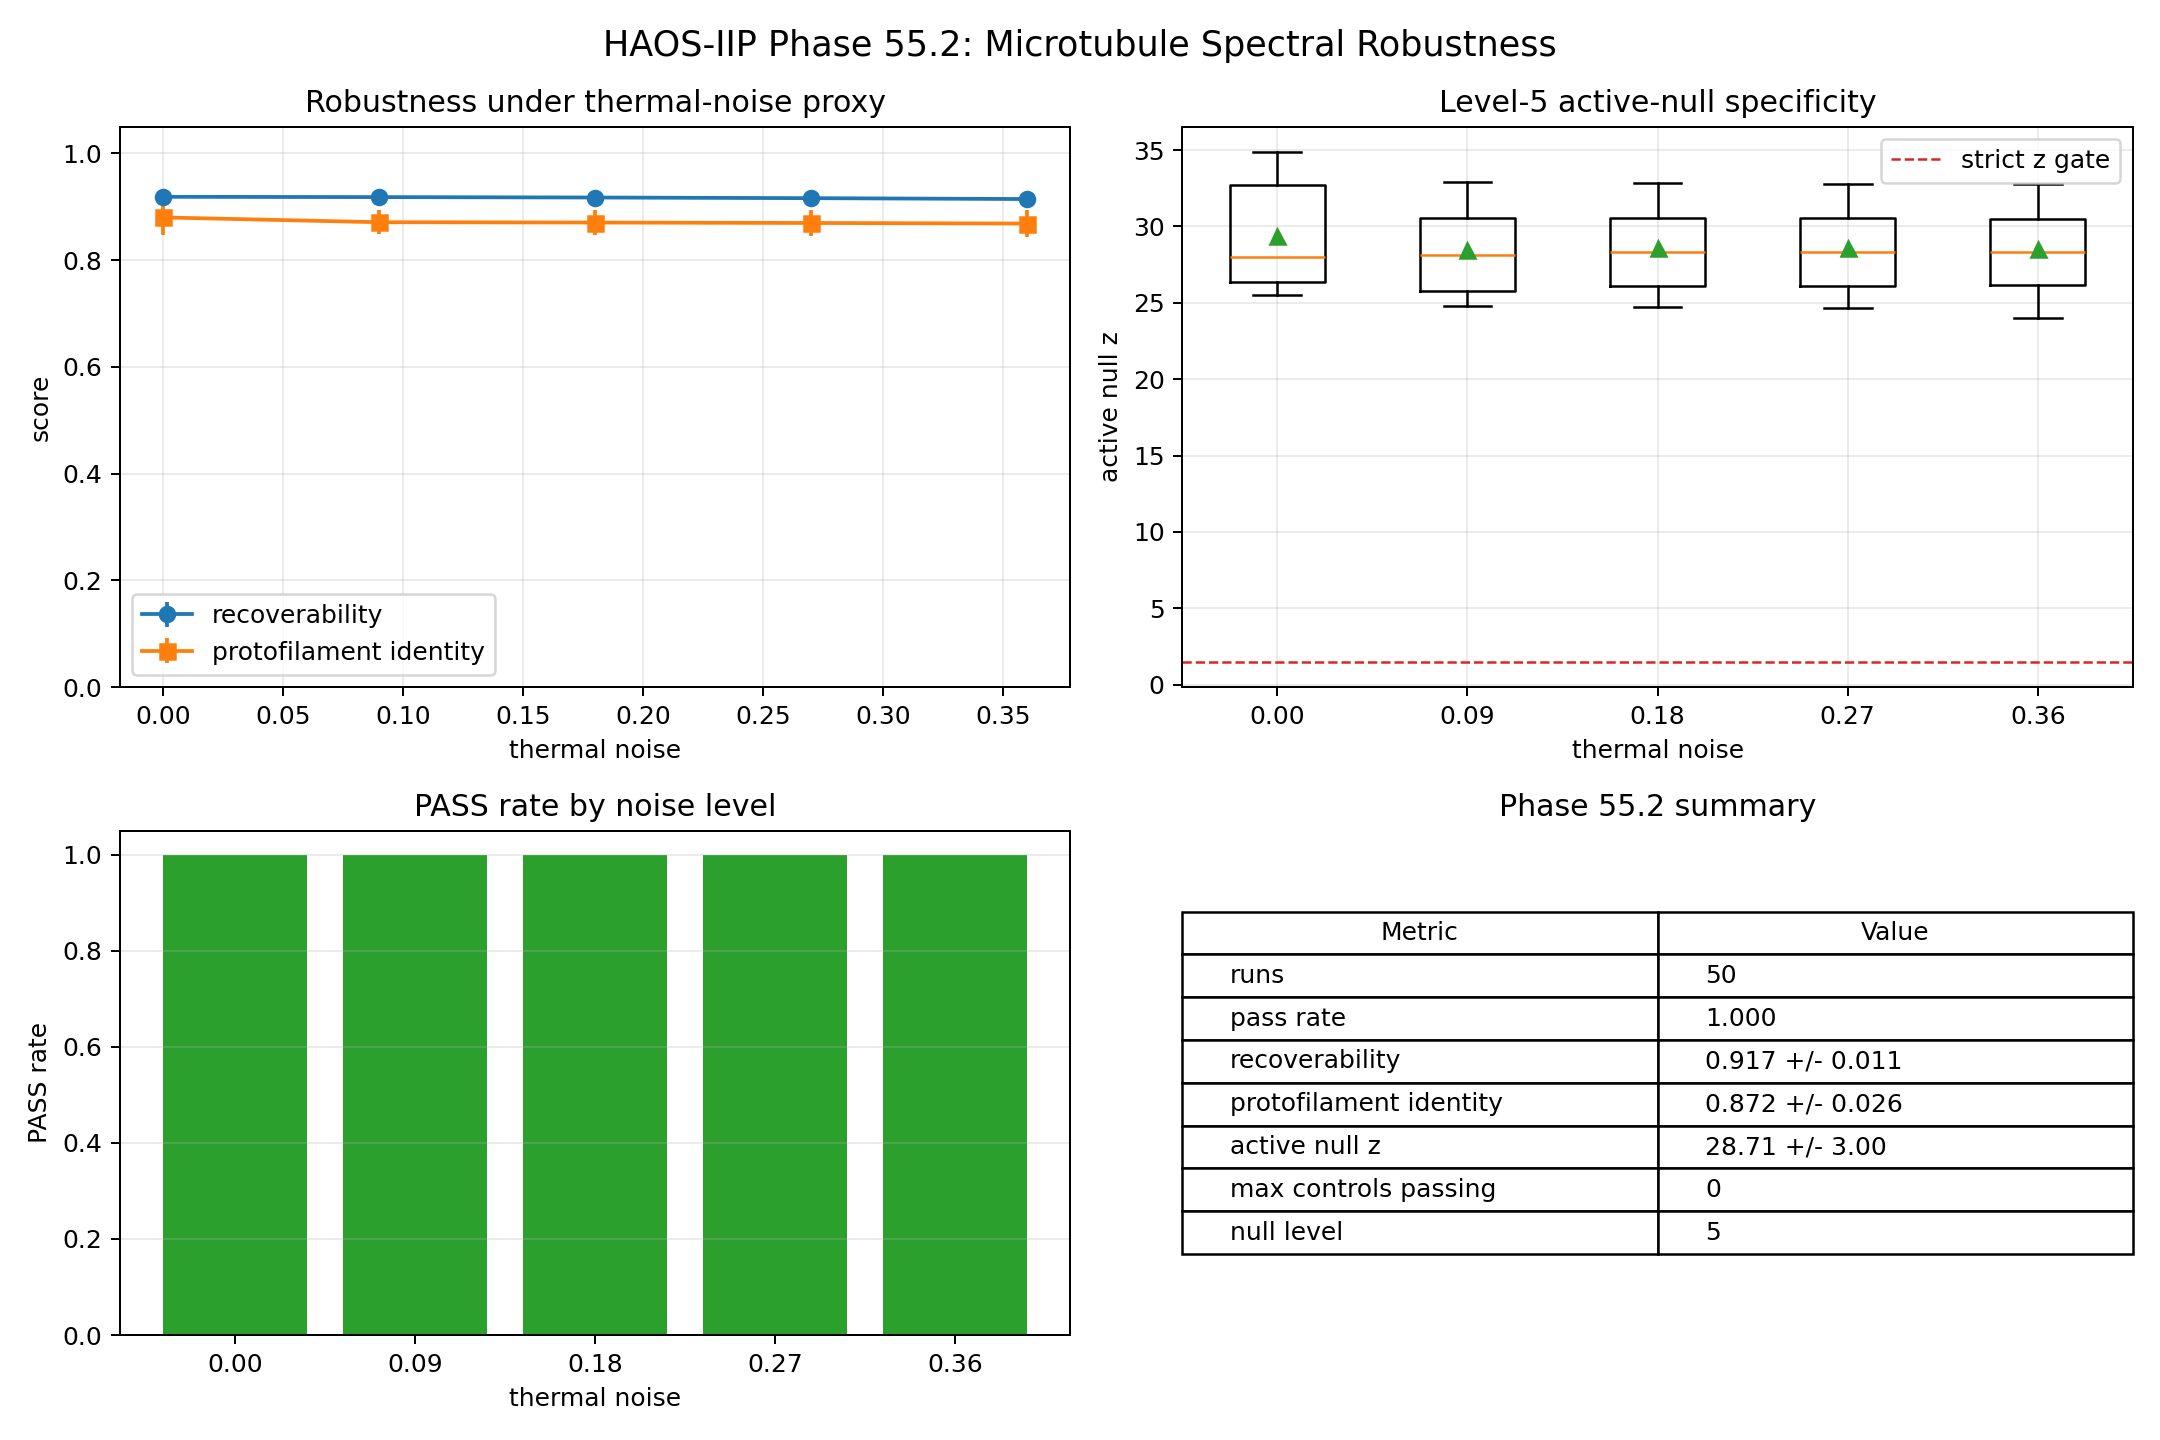
\includegraphics[width=\linewidth]{figures/phase55_2_microtubule_robustness_visual_summary.png}
\caption{Phase 55.2 visual summary. The 50-run microtubule robustness sweep keeps recoverability and protofilament identity high across the tested thermal-noise proxy levels, while the level-5 trajectory-aware null remains well above the strict specificity gate and no controls pass.}
\end{figure}

\section{Scope and Boundary}

This paper freezes a sidecar result, not a core HAOS-IIP phase. The implementation lives under:
\begin{quote}
\texttt{experiments/dynamics/haos\_minimal\_dynamics/}

\texttt{experiments/biology/microtubule\_lattice\_demo/}
\end{quote}

The scope is narrow:
\begin{itemize}
\item test whether spectral-address dynamics preserve recoverable structure under perturbation;
\item harden specificity tests through a null ladder;
\item apply the resulting telemetry instrument to a microtubule-inspired toy lattice;
\item keep all biological interpretation bounded and falsifiable.
\end{itemize}

This release does not modify the frozen HAOS-IIP core. It does not assert a physical derivation of microtubule behavior, spacetime, quantum computation, Orch-OR, or consciousness.

\section{Spectral Address Dynamics}

The minimal dynamics probe began with a scalar state $x_t$ on a weighted graph:
\[
x_{t+1}
= x_t - \Delta t\,D L x_t
+ \Delta t\,A\,\mathcal{R}_{address}(x_t)
+ \Delta t\,I\,\mathcal{R}_{shell}(x_t).
\]

The original address restoration used local neighbor-difference recovery. Targeted ablations showed that this local term was weak: removing it did not substantially degrade strict branch-identity specificity. The address term was therefore refactored into selectable modes:
\begin{itemize}
\item local neighbor-difference restoration;
\item spectral projection onto low-frequency frozen Laplacian modes;
\item hybrid spectral/local restoration;
\item scalar phase-style restoration;
\item shell-weighted multi-scale restoration.
\end{itemize}

The spectral version became the default. The default address gain was promoted to $0.45$ after a fixed gain sweep. On the internal minimal graph probe, the upgraded default reports:
\begin{center}
\begin{tabular}{lr}
\toprule
Metric & Value \\
\midrule
recoverability score & 0.894686 \\
branch identity $z$ & 13.987830 \\
spectral-aware $z$ & 10.173756 \\
autocorrelation-aware $z$ & 11.029351 \\
higher-order $z$ & 9.094737 \\
trajectory-aware $z$ & 12.909551 \\
\bottomrule
\end{tabular}
\end{center}

The internal status remains marginal because all controls still pass the strict gates. This is retained as a negative/diagnostic result.

\section{Null Ladder}

The specificity tests were hardened into a five-level null ladder:
\begin{center}
\begin{tabular}{clp{0.58\linewidth}}
\toprule
Level & Name & Preserved structure \\
\midrule
1 & degree/shell & weighted degree and frozen shell-variance buckets \\
2 & spectral-aware & level 1 plus low-mode spectral energy matching \\
3 & autocorrelation-aware & level 2 plus one-hop local autocorrelation matching \\
4 & higher-order & level 3 plus two-hop and triangle-supported correlation proxies \\
5 & trajectory-aware & level 4 plus compact state-transition and lag-profile statistics \\
\bottomrule
\end{tabular}
\end{center}

The null ladder did not produce a decisive internal PASS on the abstract graph. It did produce a more precise failure mode: the abstract dynamics preserve strong recoverable structure, but not a uniquely branch-local identity signature under correlation-preserving controls.

\section{Microtubule Spectral Telemetry Prototype}

The external sidecar uses a microtubule-inspired cylindrical graph with 13 protofilaments and 30 longitudinal sites per protofilament. The graph contains longitudinal, lateral, diagonal, and weak-support couplings inherited from the existing Biology Line B lattice model. A toy reference field combines:
\begin{itemize}
\item helical phase variation around the cylinder;
\item lateral protofilament modulation;
\item a cap-like distal enrichment.
\end{itemize}

The spectral dynamics are run under a localized cap-region perturbation and small thermal-noise proxy. The telemetry reports:
\begin{itemize}
\item recoverability score;
\item protofilament identity retention;
\item delta persistence;
\item safety margin;
\item active null $z$;
\item control pass counts.
\end{itemize}

The default command is:
\begin{quote}
\texttt{uv run --with numpy --with matplotlib python experiments/biology/microtubule\_lattice\_demo/run\_microtubule\_spectral\_telemetry.py}
\end{quote}

\section{Default Result}

The default run gives:
\begin{center}
\begin{tabular}{lr}
\toprule
Metric & Value \\
\midrule
nodes & 390 \\
edges & 1193 \\
null level & 4 \\
recoverability score & 0.913607 \\
protofilament identity retention & 0.830157 \\
delta persistence & 0.050835 \\
active null $z$ & 30.910884 \\
control strict pass count & 0 \\
\bottomrule
\end{tabular}
\end{center}

The control comparison is:
\begin{center}
\begin{tabular}{lrrrr}
\toprule
Run & Recoverability & Protofilament identity & Active null $z$ & Strict pass \\
\midrule
observed & 0.913607 & 0.830157 & 30.910884 & true \\
node shuffle & 0.393491 & 0.000000 & 23.219667 & false \\
edge shuffle & 0.646325 & 0.696868 & 23.060728 & false \\
topology randomization & 0.622533 & 0.695210 & 11.743433 & false \\
\bottomrule
\end{tabular}
\end{center}

Level 5 trajectory-aware nulls also pass in the observed run with zero controls passing.

\section{Phase 55.2 Robustness Sweep}

A 50-run robustness sweep over ten deterministic seeds and five thermal-noise proxy levels was added:
\begin{quote}
\texttt{uv run --with numpy --with matplotlib python experiments/biology/microtubule\_lattice\_demo/run\_microtubule\_robustness.py --seed-count 10 --thermal-noise 0.00,0.09,0.18,0.27,0.36 --permutation-trials 32 --null-candidates 2}
\end{quote}

It reports:
\begin{center}
\begin{tabular}{lr}
\toprule
Metric & Value \\
\midrule
runs & 50 \\
pass rate & 1.000000 \\
recoverability mean & 0.916789 \\
recoverability std & 0.011193 \\
protofilament identity mean & 0.871810 \\
protofilament identity std & 0.026071 \\
active null $z$ mean & 28.705018 \\
active null $z$ std & 3.000322 \\
control pass maximum & 0 \\
\bottomrule
\end{tabular}
\end{center}

Across the tested noise ladder, all five noise levels preserve a 1.000000 pass rate. The worst observed recoverability across all 50 runs is $0.897014$, and the worst observed protofilament identity retention is $0.824970$.

\section{Interpretation}

The internal graph probe and the microtubule sidecar should be read together. The internal probe shows that spectral dynamics alone are not enough to guarantee unique branch identity on arbitrary or reconstructed graphs. The microtubule sidecar shows that the same instrument can produce a clean external toy PASS when the substrate has a strong cylindrical, multi-scale coupling structure.

The bounded conclusion is therefore:
\begin{quote}
Spectral HAOS-style dynamics plus hardened null telemetry can identify recoverable protofilament-level structure in a microtubule-inspired toy lattice, while remaining honest about marginal specificity on abstract internal graphs.
\end{quote}

\section{Open Limits}

\begin{itemize}
\item The microtubule model is a toy graph, not a molecular simulation.
\item The cap-like field is an engineered reference, not an experimental GTP cap measurement.
\item The noise model is a computational perturbation proxy, not thermal physics.
\item The robustness sweep is still parameter-bounded: it scans the thermal-noise proxy, but not lattice size, damage geometry, address mode, or molecular-scale model variants.
\item The spectral dynamics perform more decisively on structured cylindrical lattices than on abstract internal graphs. This suggests sensitivity to interaction architecture, not a general proof of unique branch identity on arbitrary substrates.
\item No biological, quantum, or consciousness claim follows from this result.
\end{itemize}

\section{Next Work}

The natural next work is:
\begin{itemize}
\item run larger multi-seed sweeps;
\item scan thermal noise and damage scale to estimate safety margins;
\item test larger lattices such as $13 \times 60$ and $13 \times 100$;
\item compare spectral, local, and hybrid address modes on the same lattice;
\item add a second biology telemetry prototype for contrast.
\end{itemize}

\section{Release Artifacts}

Primary artifacts:
\begin{itemize}
\item \texttt{experiments/biology/microtubule\_lattice\_demo/microtubule\_spectral\_telemetry.py}
\item \texttt{experiments/biology/microtubule\_lattice\_demo/run\_microtubule\_spectral\_telemetry.py}
\item \texttt{experiments/biology/microtubule\_lattice\_demo/run\_microtubule\_spectral\_sweep.py}
\item \texttt{experiments/biology/microtubule\_lattice\_demo/run\_microtubule\_robustness.py}
\item \texttt{experiments/dynamics/haos\_minimal\_dynamics/haos\_minimal\_dynamics.py}
\end{itemize}

The result is a sidecar release and should be judged by reproducibility, control behavior, and bounded interpretation rather than by speculative extrapolation.

\end{document}
